\section{Paper 4}

\title[PhD Defence]{
    {\Huge Paper 4} \\
    \vspace{2mm}
    {\Large Stability of Linear Systems under\\Extended Weakly-Hard Constraints} \\
}
\author[Nils Vreman]{
    Nils Vreman \\
    \vspace{3mm}
    {\large Paolo Pazzaglia, Victor Magron, Jie Wang, Martina Maggio}
}
\date[LCSS 2022]{
    Control Systems Letters, 2022\\
}
\notitlelogo
\frame[plain,noframenumbering]{\titlepage}


\begin{frame}
    \frametitle{Extended Weakly-Hard Model}%
    \framesubtitle{Problem}%
    \begin{figure}[h]
        \centering
        \only<1>{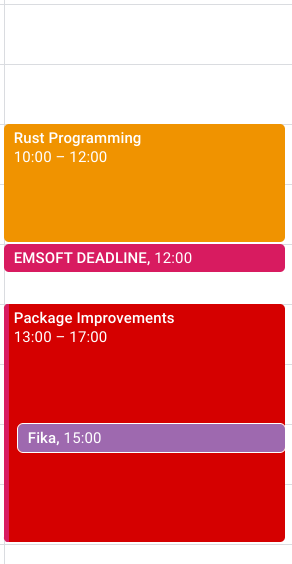
\includegraphics[width=0.25\textwidth]{figs/topic/small-schedule-kill.png}}%
        \only<2>{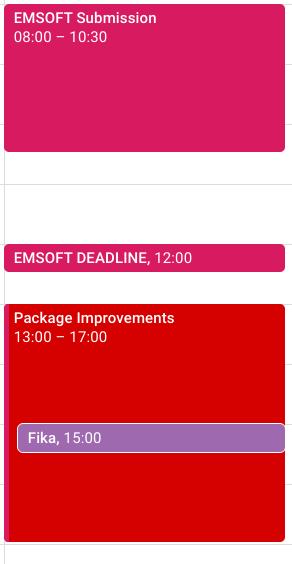
\includegraphics[width=0.25\textwidth]{figs/topic/small-schedule-skip.png}}%
    \end{figure}
\end{frame}

\begin{frame}
    \frametitle{Extended Weakly-Hard Model}
    \framesubtitle<1>{Problem}%
    \framesubtitle<2>{Solution}%
    \begin{minipage}[c]{0.23\textwidth}
        \centering
        \begin{equation*}
            \begin{matrix}
                \only<1>{\Large \anyhit{}}%
                \only<2>{\Large \anyhit{}^{\textcolor{hicolour}{\strat}}}\\
                            \\
                \tAH{}
            \end{matrix}
        \end{equation*}\newline
    \end{minipage}\hfill
    \begin{minipage}[c]{0.23\textwidth}
        \centering
        \begin{equation*}
            \begin{matrix}
                \only<1>{\Large \anymiss{}}%
                \only<2>{\Large \anymiss{}^{\textcolor{hicolour}{\strat}}}\\
                            \\
                \tAM{}
            \end{matrix}
        \end{equation*}\newline
    \end{minipage}\hfill
    \begin{minipage}[c]{0.23\textwidth}
        \centering
        \begin{equation*}
            \begin{matrix}
                \only<1>{\Large \rowhit{}}%
                \only<2>{\Large \rowhit{}^{\textcolor{hicolour}{\strat}}}\\
                            \\
                \tRH{}
            \end{matrix}
        \end{equation*}\newline
    \end{minipage}\hfill
    \begin{minipage}[c]{0.23\textwidth}
        \centering
        \begin{equation*}
            \begin{matrix}
                \only<1>{\Large \rowmiss{}}%
                \only<2>{\Large \rowmiss{}^{\textcolor{hicolour}{\strat}}}\\
                            \\
                \tRM{}
            \end{matrix}
        \end{equation*}\newline
    \end{minipage}

    \centering
    \only<1>{%
        \textcolor{red}{Deadline hits/misses}
    }%
    \only<2>{%
        \textcolor{hicolour}{Job completions/overruns}
    }%
\end{frame}


\begin{frame}
    \frametitle{Discrete Switched Linear Systems}%
    \framesubtitle{Arbitrary Switching}%
    \begin{figure}[h]
        \centering
        \only<1>{\def \delta {0.15}
\def \armlength {0.625}
\def \armwidthcm {0.1cm}
\def \bodywidthcm {0.5cm}
\def \circlesizecm {0.5cm}
\def \circleshiftcm {0.125cm}

\begin{tikzpicture}

\tikzstyle{task} = [draw,thick,fill=white,align=center]
\tikzstyle{eng-step} = [draw, thick, fill=white, align=center, minimum width=1.5cm, minimum height=1.5cm]
\tikzstyle{turbine} = [circle,ultra thick,draw,fill=white,minimum size=\circlesizecm,inner sep=0pt,outer sep=0pt]

%%% Controllers %%%

\node[eng-step, opacity=0.1] (c4) at (-1.10-3*\delta, 3*\delta) {\textcolor{white}{\Huge$\mathcal{C}$}};
\node[eng-step, opacity=0.4] (c3) at (-1.10-2*\delta, 2*\delta) {\textcolor{white}{\Huge$\mathcal{C}$}};
\node[eng-step, opacity=0.7] (c2) at (-1.10-1*\delta, 1*\delta) {\textcolor{white}{\Huge$\mathcal{C}$}};
\node[eng-step] (c1) at (-1.10-0*\delta, 0*\delta) {\Huge$\mathcal{C}$};
\coordinate (c) at (-2.75, 0);

%%%% Plant %%%
\node[task, minimum width=2.125cm, minimum height=2.125cm] (phys) at (2.5,0) {};
% body
\node[
    draw,
    rounded corners=3pt,
    fill=black,
    minimum width=\bodywidthcm,
    minimum height=\bodywidthcm,
    name path=B] (body) at (phys) {};

% upper left turbine
\node[turbine, anchor=south east] (dronenw) at ([xshift=-\circleshiftcm, yshift=\circleshiftcm]body.north west) {};
\draw[name path=NW] ([yshift=-\armwidthcm]body.north west)..controls($(phys) + (-\armlength, \armlength)$)..([xshift=\armwidthcm]body.north west);
\tikzfillbetween [of=NW and B] {};
\draw[fill=black, rotate=75] (dronenw) ellipse (0.175cm and 0.025cm);
\draw[fill=black, rotate=165] (dronenw) ellipse (0.175cm and 0.025cm);
        
% upper right turbine
\node[turbine, anchor=south west] (dronene) at ([xshift=\circleshiftcm, yshift=\circleshiftcm]body.north east) {};
\draw[name path=NE] ([xshift=-\armwidthcm]body.north east)..controls($(phys) + (\armlength, \armlength)$)..([yshift=-\armwidthcm]body.north east);
\tikzfillbetween [of=NE and B] {};
\draw[fill=black, rotate=75] (dronene) ellipse (0.175cm and 0.025cm);
\draw[fill=black, rotate=165] (dronene) ellipse (0.175cm and 0.025cm);

% lower right turbine
\node[turbine, anchor=north west] (dronese) at ([xshift=\circleshiftcm, yshift=-\circleshiftcm]body.south east) {};
\draw[name path=SE] ([yshift=\armwidthcm]body.south east)..controls($(phys) + (\armlength, -\armlength)$)..([xshift=-\armwidthcm]body.south east);
\tikzfillbetween [of=SE and B] {};
\draw[fill=black, rotate=75] (dronese) ellipse (0.175cm and 0.025cm);
\draw[fill=black, rotate=165] (dronese) ellipse (0.175cm and 0.025cm);

% lower left turbine
\node[turbine, anchor=north east] (dronesw) at ([xshift=-\circleshiftcm, yshift=-\circleshiftcm]body.south west) {};
\draw[name path=SW] ([xshift=\armwidthcm]body.south west)..controls($(phys) + (-\armlength, -\armlength)$)..([yshift=\armwidthcm]body.south west);
\tikzfillbetween [of=SW and B] {};
\draw[fill=black, rotate=75] (dronesw) ellipse (0.175cm and 0.025cm);
\draw[fill=black, rotate=165] (dronesw) ellipse (0.175cm and 0.025cm);

\coordinate (p2) at (4.0, -1.5);

%%%%%%%%%%%%%%%
%%%% ARROWS %%%
%%%%%%%%%%%%%%%

\draw[-latex,thick] (c1.east) to (phys.west);

\draw[-,thick] (phys.east)  -| (p2) -| (c);

\draw[-latex,thick] (c) to (c1.west);

\end{tikzpicture}
}%
        \only<2>{\begin{tikzpicture}
\tikzstyle{eng-step} = [draw, thick, fill=white, align=center, minimum width=1cm, minimum height=1cm]


%%% Switch %%%

\coordinate (s) at (-1.0, 0);
\node[eng-step, rotate=270] (switch)  at (0, 0) {\Large \faSitemap};

%%% Controllers %%%

\node[eng-step] (c2) at (-2.25, 0.15) {\Large$\mathcal{C}$};
\node[eng-step, draw=lqgcolour] (c1) at (-2.10, 0) {\textcolor{lqgcolour}{\Large$\mathcal{C}$}};
\coordinate (c) at (-4, 0);

%%%% Plant %%%

\node[eng-step] (plant)     at (2.5,0) {\Large$\mathcal{P}$};
\coordinate (p2) at (4, -2);

%%%%%%%%%%%%%%%
%%%% ARROWS %%%
%%%%%%%%%%%%%%%

\draw[-latex,thick] (c1.east) to (switch.south);

\draw[-latex,thick] (switch.north) to (plant.west);

\draw[-,thick] (plant.east)  -| (p2) -| (c);

\draw[-latex,thick] (c) to (c1.west);

\end{tikzpicture}
}%
        \only<3>{\begin{tikzpicture}
\tikzstyle{eng-step} = [draw, thick, fill=white, align=center, minimum width=1cm, minimum height=1cm]


%%% Switch %%%

\coordinate (s) at (-1.0, 0);
\node[eng-step, rotate=270] (switch)  at (0, 0) {\Large \faSitemap};

%%% Controllers %%%

\node[eng-step, draw=red!80!black] (c2) at (-2.25, 0.15) {\textcolor{red!80!black}{\Large$\mathcal{C}$}};
\node[eng-step, draw=lqgcolour] (c1) at (-2.10, 0) {\textcolor{lqgcolour}{\Large$\mathcal{C}$}};
\coordinate (c) at (-4, 0);

%%%% Plant %%%

\node[eng-step] (plant)     at (2.5,0) {\Large$\mathcal{P}$};
\coordinate (p2) at (4, -2);

%%%%%%%%%%%%%%%
%%%% ARROWS %%%
%%%%%%%%%%%%%%%

\draw[-latex,thick] (c1.east) to (switch.south);

\draw[-latex,thick] (switch.north) to (plant.west);

\draw[-,thick] (plant.east)  -| (p2) -| (c);

\draw[-latex,thick] (c) to (c1.west);

\end{tikzpicture}
}%
        \only<4>{\def \delta {0.15}
\def \armlength {0.625}
\def \armwidthcm {0.1cm}
\def \bodywidthcm {0.5cm}
\def \circlesizecm {0.5cm}
\def \circleshiftcm {0.125cm}

\begin{tikzpicture}

\tikzstyle{task} = [draw,thick,fill=white,align=center]
\tikzstyle{eng-step} = [draw, thick, fill=white, align=center, minimum width=1.5cm, minimum height=1.5cm]
\tikzstyle{turbine} = [circle,ultra thick,draw,fill=white,minimum size=\circlesizecm,inner sep=0pt,outer sep=0pt]

%%% Controllers %%%

{\color{red}\node[eng-step, opacity=0.7] (c2) at (-1.10-1*\delta, 1*\delta) {\textcolor{white}{\Huge$\mathcal{C}$}};}
{\color{hicolour}\node[eng-step] (c1) at (-1.10-0*\delta, 0*\delta) {\Huge$\mathcal{C}$};}
\coordinate (c) at (-2.75, 0);

%%%% Plant %%%
\node[task, minimum width=2.125cm, minimum height=2.125cm] (phys) at (2.5,0) {};
% body
\node[
    draw,
    rounded corners=3pt,
    fill=black,
    minimum width=\bodywidthcm,
    minimum height=\bodywidthcm,
    name path=B] (body) at (phys) {};

% upper left turbine
\node[turbine, anchor=south east] (dronenw) at ([xshift=-\circleshiftcm, yshift=\circleshiftcm]body.north west) {};
\draw[name path=NW] ([yshift=-\armwidthcm]body.north west)..controls($(phys) + (-\armlength, \armlength)$)..([xshift=\armwidthcm]body.north west);
\tikzfillbetween [of=NW and B] {};
\draw[fill=black, rotate=75] (dronenw) ellipse (0.175cm and 0.025cm);
\draw[fill=black, rotate=165] (dronenw) ellipse (0.175cm and 0.025cm);
        
% upper right turbine
\node[turbine, anchor=south west] (dronene) at ([xshift=\circleshiftcm, yshift=\circleshiftcm]body.north east) {};
\draw[name path=NE] ([xshift=-\armwidthcm]body.north east)..controls($(phys) + (\armlength, \armlength)$)..([yshift=-\armwidthcm]body.north east);
\tikzfillbetween [of=NE and B] {};
\draw[fill=black, rotate=75] (dronene) ellipse (0.175cm and 0.025cm);
\draw[fill=black, rotate=165] (dronene) ellipse (0.175cm and 0.025cm);

% lower right turbine
\node[turbine, anchor=north west] (dronese) at ([xshift=\circleshiftcm, yshift=-\circleshiftcm]body.south east) {};
\draw[name path=SE] ([yshift=\armwidthcm]body.south east)..controls($(phys) + (\armlength, -\armlength)$)..([xshift=-\armwidthcm]body.south east);
\tikzfillbetween [of=SE and B] {};
\draw[fill=black, rotate=75] (dronese) ellipse (0.175cm and 0.025cm);
\draw[fill=black, rotate=165] (dronese) ellipse (0.175cm and 0.025cm);

% lower left turbine
\node[turbine, anchor=north east] (dronesw) at ([xshift=-\circleshiftcm, yshift=-\circleshiftcm]body.south west) {};
\draw[name path=SW] ([xshift=\armwidthcm]body.south west)..controls($(phys) + (-\armlength, -\armlength)$)..([yshift=\armwidthcm]body.south west);
\tikzfillbetween [of=SW and B] {};
\draw[fill=black, rotate=75] (dronesw) ellipse (0.175cm and 0.025cm);
\draw[fill=black, rotate=165] (dronesw) ellipse (0.175cm and 0.025cm);

\coordinate (p2) at (4.0, -1.5);

%%%%%%%%%%%%%%%
%%%% ARROWS %%%
%%%%%%%%%%%%%%%

\draw[-latex,thick] (c1.east) to (phys.west);

\draw[-,thick] (phys.east)  -| (p2) -| (c);

\draw[-latex,thick] (c) to (c1.west);

\end{tikzpicture}
}
    \end{figure}
\end{frame}


\begin{frame}
    \frametitle{Discrete Switched Linear Systems}
    \framesubtitle{Stability}
    \begin{itemize}\setlength\itemsep{1em}
        \item Lyapunov Theory\footnote{\cite{Liberzon:2003, Linsenmayer:2021, Hertneck:2021}}
        \item Joint Spectral Radius (JSR)\footnote{\cite{Maggio:2020, Ogura:2013}}
        \item Constrained Joint Spectral Radius (CJSR)\footnote{\cite{Dai:2012}}
    \end{itemize}
\end{frame}


\begin{frame}
    \frametitle{Discrete Switched Linear Systems}
    \framesubtitle{JSR}
    \begin{minipage}{0.59\textwidth}
        \begin{figure}[h]
            \centering
            \begin{tikzpicture}
\tikzstyle{eng-step} = [draw, thick, fill=white, align=center, minimum width=1cm, minimum height=1cm]


%%% Switch %%%

\coordinate (s) at (-1.0, 0);
\node[eng-step, rotate=270] (switch)  at (0, 0) {\Large \faSitemap};

%%% Controllers %%%

\node[eng-step, draw=red!80!black] (c2) at (-2.25, 0.15) {\textcolor{red!80!black}{\Large$\mathcal{C}$}};
\node[eng-step, draw=lqgcolour] (c1) at (-2.10, 0) {\textcolor{lqgcolour}{\Large$\mathcal{C}$}};
\coordinate (c) at (-4, 0);

%%%% Plant %%%

\node[eng-step] (plant)     at (2.5,0) {\Large$\mathcal{P}$};
\coordinate (p2) at (4, -2);

%%%%%%%%%%%%%%%
%%%% ARROWS %%%
%%%%%%%%%%%%%%%

\draw[-latex,thick] (c1.east) to (switch.south);

\draw[-latex,thick] (switch.north) to (plant.west);

\draw[-,thick] (plant.east)  -| (p2) -| (c);

\draw[-latex,thick] (c) to (c1.west);

\end{tikzpicture}

        \end{figure}
    \end{minipage}\hfill
    \begin{minipage}{0.39\textwidth}
        \begin{figure}[h]
            \centering
            \begin{tikzpicture}[>=latex]
                \node[Init Node] (a) at (0,0) {$1$};
                \node[Dom Node] (b) at (0,-1.75) {$10$};
                \node[Dom Node] (c) at (0,-3.5) {$100$};
                \draw[->] (a) edge [loop above] node[above] {$1$} (a);
                \draw[->] (a) edge [bend left=67.5] node[right] {$0$} (b);
                \draw[->] (b) edge [bend left=50] node[right] {$1$} (a);
                \draw[->] (b) edge [bend left=67.5] node[right] {$0$} (c);
                \draw[->] (c) edge [bend left=57.5] node[left] {$1$} (a);
            \end{tikzpicture}
        \end{figure}
    \end{minipage}

    \begin{minipage}{0.59\textwidth}
        \centering
        \large
        $\mathcal{A} = \left\{ \;\textcolor{red}{A_{\texttt{M}}}, \,\textcolor{hicolour}{A_{\texttt{H}}}\; \right\}$
    \end{minipage}\hfill
    \begin{minipage}{0.39\textwidth}
        \centering
        \large
        Ex.: $\dots \,\textcolor{red}{0} \, \textcolor{hicolour}{1} \, \textcolor{red}{0} \, \textcolor{red}{0} \, \textcolor{hicolour}{1} \, \textcolor{hicolour}{1}\, \textcolor{red}{0} \,\dots$
    \end{minipage}
\end{frame}


\begin{frame}
    \frametitle{Discrete Switched Linear Systems}
    \framesubtitle{JSR}
    \begin{figure}[h]
        \centering
        \def \delta {0.15}
\def \armlength {0.625}
\def \armwidthcm {0.1cm}
\def \bodywidthcm {0.5cm}
\def \circlesizecm {0.5cm}
\def \circleshiftcm {0.125cm}

\begin{tikzpicture}

\tikzstyle{task} = [draw,thick,fill=white,align=center]
\tikzstyle{eng-step} = [draw, thick, fill=white, align=center, minimum width=1.5cm, minimum height=1.5cm]
\tikzstyle{turbine} = [circle,ultra thick,draw,fill=white,minimum size=\circlesizecm,inner sep=0pt,outer sep=0pt]

%%% Controllers %%%

\node[scale=1.0] (c1) at (-1.10, 0) {%
    \begin{tikzpicture}[>=latex]
        \node[Init Node] (a) at (0,0) {$1$};
        \node[Dom Node] (b) at (0,-1.75) {$10$};
        \node[Dom Node] (c) at (0,-3.5) {$100$};
        \draw[->] (a) edge [loop above] node[above]     {\Large\textcolor{lqgcolour}{$\mathcal{C}$}} (a);
        \draw[->] (a) edge [bend left=67.5] node[right] {\Large\textcolor{red!80!black}{$\mathcal{C}$}} (b);
        \draw[->] (b) edge [bend left=50] node[right]   {\Large\textcolor{lqgcolour}{$\mathcal{C}$}} (a);
        \draw[->] (b) edge [bend left=67.5] node[right] {\Large\textcolor{red!80!black}{$\mathcal{C}$}} (c);
        \draw[->] (c) edge [bend left=57.5] node[left]  {\Large\textcolor{lqgcolour}{$\mathcal{C}$}} (a);
    \end{tikzpicture}%
};

\coordinate (c) at (-3.25, 0);

%%%% Plant %%%
\node[task, minimum width=2.125cm, minimum height=2.125cm] (phys) at (2.5,0) {};
% body
\node[
    draw,
    rounded corners=3pt,
    fill=black,
    minimum width=\bodywidthcm,
    minimum height=\bodywidthcm,
    name path=B] (body) at (phys) {};

% upper left turbine
\node[turbine, anchor=south east] (dronenw) at ([xshift=-\circleshiftcm, yshift=\circleshiftcm]body.north west) {};
\draw[name path=NW] ([yshift=-\armwidthcm]body.north west)..controls($(phys) + (-\armlength, \armlength)$)..([xshift=\armwidthcm]body.north west);
\tikzfillbetween [of=NW and B] {};
\draw[fill=black, rotate=75] (dronenw) ellipse (0.175cm and 0.025cm);
\draw[fill=black, rotate=165] (dronenw) ellipse (0.175cm and 0.025cm);
        
% upper right turbine
\node[turbine, anchor=south west] (dronene) at ([xshift=\circleshiftcm, yshift=\circleshiftcm]body.north east) {};
\draw[name path=NE] ([xshift=-\armwidthcm]body.north east)..controls($(phys) + (\armlength, \armlength)$)..([yshift=-\armwidthcm]body.north east);
\tikzfillbetween [of=NE and B] {};
\draw[fill=black, rotate=75] (dronene) ellipse (0.175cm and 0.025cm);
\draw[fill=black, rotate=165] (dronene) ellipse (0.175cm and 0.025cm);

% lower right turbine
\node[turbine, anchor=north west] (dronese) at ([xshift=\circleshiftcm, yshift=-\circleshiftcm]body.south east) {};
\draw[name path=SE] ([yshift=\armwidthcm]body.south east)..controls($(phys) + (\armlength, -\armlength)$)..([xshift=-\armwidthcm]body.south east);
\tikzfillbetween [of=SE and B] {};
\draw[fill=black, rotate=75] (dronese) ellipse (0.175cm and 0.025cm);
\draw[fill=black, rotate=165] (dronese) ellipse (0.175cm and 0.025cm);

% lower left turbine
\node[turbine, anchor=north east] (dronesw) at ([xshift=-\circleshiftcm, yshift=-\circleshiftcm]body.south west) {};
\draw[name path=SW] ([xshift=\armwidthcm]body.south west)..controls($(phys) + (-\armlength, -\armlength)$)..([yshift=\armwidthcm]body.south west);
\tikzfillbetween [of=SW and B] {};
\draw[fill=black, rotate=75] (dronesw) ellipse (0.175cm and 0.025cm);
\draw[fill=black, rotate=165] (dronesw) ellipse (0.175cm and 0.025cm);

\coordinate (p2) at (4.0, -3.5);

%%%%%%%%%%%%%%%
%%%% ARROWS %%%
%%%%%%%%%%%%%%%

\draw[-latex,thick] (c1.east) to (phys.west);

\draw[-,thick] (phys.east)  -| (p2) -| (c);

\draw[-latex,thick] (c) to (c1.west);

\end{tikzpicture}

    \end{figure}
\end{frame}
